\documentclass{article}
\usepackage{tikz}
\usepackage{amsmath}
\usepackage{graphicx}
\usepackage{hyperref}
\usepackage{geometry}
\geometry{margin=1in}

\title{INSURE-AI: A National-Interest AI Modernization Methodology for Insurance Systems}
\author{Rohin Solan}
\date{2026}

\begin{document}
\maketitle

\begin{abstract}
The insurance industry is a critical component of national economic stability and public resilience, yet many insurance systems still rely on legacy technology, fragmented data, and ad hoc analytics. This paper introduces INSURE-AI, a novel applied AI modernization methodology designed specifically for insurance systems operating under national-interest constraints. INSURE-AI defines a structured, six-phase approach that integrates data mining, enterprise machine learning (ML) pipelines, AI copilots, and low-code automation platforms into a coherent modernization strategy. The methodology emphasizes regulatory compliance, risk-aware design, and operational resilience, while leveraging modern AI capabilities to improve claims processing, fraud detection, underwriting, and customer experience. We present the conceptual framework, reference architecture, and example workflows using ML pipelines, Copilot integration, and Power Platform automation. The result is a unique, domain-specific methodology that guides insurers in transforming their technology stack in a way that is technically robust, economically viable, and aligned with national-interest priorities.
\end{abstract}

\textbf{Keywords:} data mining, machine learning, pipelines, Copilot, Power Platform, insurance, national interest, INSURE-AI, LLMOps, MLOps

\section{Introduction}
Insurance organizations operate at the intersection of financial stability, public safety, and regulatory oversight. Claims, policies, underwriting decisions, and fraud investigations generate large volumes of structured and unstructured data. Traditional systems often struggle to process this data efficiently, leading to delays, inaccuracies, and increased operational risk.

Recent advances in AI, including large language models (LLMs), enterprise ML pipelines, and low-code automation platforms, create an opportunity to modernize insurance operations. However, the adoption of these technologies must be guided by a methodology that respects national-interest constraints, regulatory requirements, and the unique risk profile of insurance systems.

This paper proposes INSURE-AI, a new applied AI modernization methodology tailored to insurance. INSURE-AI provides a structured approach to integrating data mining, ML pipelines, Copilot-style AI assistants, and Power Platform automation into insurance workflows, while maintaining compliance, resilience, and governance.

\section{The INSURE-AI Methodology}
INSURE-AI is defined as a six-phase methodology, with each phase addressing a specific dimension of AI modernization in insurance systems. The acronym INSURE captures the core steps:

\begin{itemize}
    \item \textbf{I -- Identify National-Interest Objectives}
    \item \textbf{N -- Normalize and Mine Enterprise Data}
    \item \textbf{S -- Structure ML Pipelines for Regulated Environments}
    \item \textbf{U -- Unify Human + Copilot Collaboration}
    \item \textbf{R -- Reinforce Automation with Power Platform}
    \item \textbf{E -- Evaluate Risk, Compliance, and Resilience}
\end{itemize}

\subsection{Phase I: Identify National-Interest Objectives}
The first phase focuses on aligning AI modernization with national-interest priorities. For insurance systems, this includes:

\begin{itemize}
    \item Ensuring continuity of operations during large-scale events (natural disasters, pandemics).
    \item Protecting sensitive customer and claims data.
    \item Maintaining financial stability and solvency.
    \item Supporting regulatory reporting and oversight.
\end{itemize}

In this phase, organizations define explicit objectives such as reducing claims processing time, improving fraud detection accuracy, and enhancing disaster response capabilities. These objectives become the guiding constraints for subsequent phases.

\subsection{Phase N: Normalize and Mine Enterprise Data}
Insurance data is often siloed across claims systems, policy administration platforms, customer relationship management tools, and external data sources. Phase N focuses on:

\begin{itemize}
    \item Data normalization across heterogeneous systems.
    \item Data quality assessment and remediation.
    \item Application of data mining techniques to extract signals from claims, policies, and interactions.
\end{itemize}

Techniques include natural language processing (NLP) for adjuster notes, entity extraction from medical reports, and pattern detection in historical claims for fraud indicators.

\subsection{Phase S: Structure ML Pipelines for Regulated Environments}
Phase S defines how ML pipelines are designed, deployed, and governed in regulated insurance environments. Key elements include:

\begin{itemize}
    \item Ingestion of normalized data into feature stores.
    \item Training models for claims triage, fraud detection, and risk scoring.
    \item Validation and monitoring for model drift and performance.
    \item Governance mechanisms for auditability and explainability.
\end{itemize}

ML pipelines must be designed with clear boundaries, versioning, and traceability to satisfy regulatory and internal audit requirements.

\subsection{Phase U: Unify Human + Copilot Collaboration}
Phase U introduces AI copilots into insurance workflows. Copilots assist human workers by:

\begin{itemize}
    \item Summarizing complex claims and documents.
    \item Suggesting next best actions for adjusters and underwriters.
    \item Drafting communications and reports.
\end{itemize}

INSURE-AI emphasizes human-in-the-loop design, where copilots augment rather than replace human judgment. This phase defines collaboration patterns, escalation rules, and guardrails for AI-generated content.

\subsection{Phase R: Reinforce Automation with Power Platform}
Phase R leverages low-code platforms such as Power Platform to automate workflows around ML and Copilot outputs. Examples include:

\begin{itemize}
    \item Power Automate flows that route high-risk claims to specialized teams.
    \item Power Apps for field adjusters to capture structured data and trigger ML predictions.
    \item Power BI dashboards for real-time monitoring of claims, fraud alerts, and operational metrics.
\end{itemize}

This phase connects AI capabilities to operational processes, ensuring that insights translate into action.

\subsection{Phase E: Evaluate Risk, Compliance, and Resilience}
The final phase focuses on continuous evaluation of:

\begin{itemize}
    \item Model risk and performance.
    \item Compliance with regulations and internal policies.
    \item Operational resilience under stress scenarios.
\end{itemize}

INSURE-AI recommends periodic reviews, scenario testing, and alignment with national-interest objectives defined in Phase I. This closes the loop and ensures that modernization remains sustainable and responsible.

\section{Reference ML Pipeline Architecture}
This section presents a reference ML pipeline architecture for insurance systems following INSURE-AI.

\subsection{Conceptual Pipeline}
The pipeline includes stages for data ingestion, feature engineering, model training, inference, and monitoring. Figure~\ref{fig:mlpipeline} shows a simplified TikZ diagram.

\begin{figure}[h]
\centering
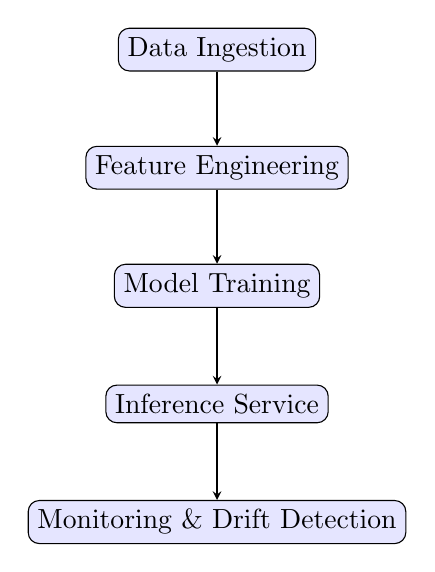
\begin{tikzpicture}[node distance=1.5cm,>=stealth]
\node[draw, rectangle, rounded corners, fill=blue!10] (ingest) {Data Ingestion};
\node[draw, rectangle, rounded corners, fill=blue!10, below of=ingest] (feature) {Feature Engineering};
\node[draw, rectangle, rounded corners, fill=blue!10, below of=feature] (train) {Model Training};
\node[draw, rectangle, rounded corners, fill=blue!10, below of=train] (infer) {Inference Service};
\node[draw, rectangle, rounded corners, fill=blue!10, below of=infer] (monitor) {Monitoring \& Drift Detection};

\draw[->] (ingest) -- (feature);
\draw[->] (feature) -- (train);
\draw[->] (train) -- (infer);
\draw[->] (infer) -- (monitor);
\end{tikzpicture}
\caption{Reference ML pipeline architecture for insurance systems.}
\label{fig:mlpipeline}
\end{figure}

\section{Copilot Workflow Integration}
Copilot integration follows Phase U of INSURE-AI, where human workers and AI assistants collaborate.

\subsection{Copilot Workflow Diagram}
Figure~\ref{fig:copilot} illustrates a simplified Copilot workflow in claims processing.

\begin{figure}[h]
\centering
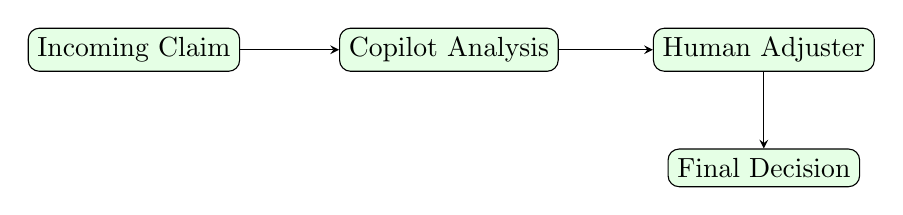
\begin{tikzpicture}[node distance=1.5cm,>=stealth]
\node[draw, rectangle, rounded corners, fill=green!10] (claim) {Incoming Claim};
\node[draw, rectangle, rounded corners, fill=green!10, right of=claim, node distance=4cm] (copilot) {Copilot Analysis};
\node[draw, rectangle, rounded corners, fill=green!10, right of=copilot, node distance=4cm] (adjuster) {Human Adjuster};
\node[draw, rectangle, rounded corners, fill=green!10, below of=adjuster] (decision) {Final Decision};

\draw[->] (claim) -- (copilot);
\draw[->] (copilot) -- (adjuster);
\draw[->] (adjuster) -- (decision);
\end{tikzpicture}
\caption{Copilot-assisted claims workflow.}
\label{fig:copilot}
\end{figure}

\section{Power Platform Automation Architecture}
Phase R of INSURE-AI uses Power Platform to reinforce automation around AI outputs.

\subsection{Automation Diagram}
Figure~\ref{fig:powerplatform} shows a conceptual automation architecture.

\begin{figure}[h]
\centering
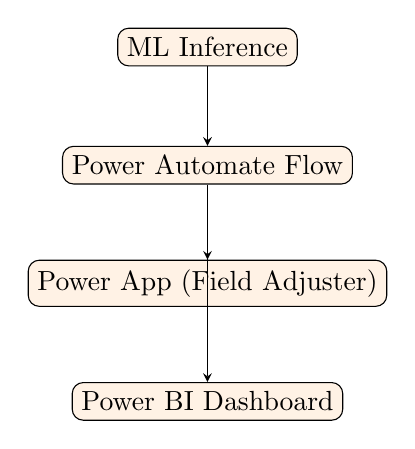
\begin{tikzpicture}[node distance=1.5cm,>=stealth]
\node[draw, rectangle, rounded corners, fill=orange!10] (ml) {ML Inference};
\node[draw, rectangle, rounded corners, fill=orange!10, below of=ml] (flow) {Power Automate Flow};
\node[draw, rectangle, rounded corners, fill=orange!10, below of=flow] (app) {Power App (Field Adjuster)};
\node[draw, rectangle, rounded corners, fill=orange!10, below of=app] (bi) {Power BI Dashboard};

\draw[->] (ml) -- (flow);
\draw[->] (flow) -- (app);
\draw[->] (flow) -- (bi);
\end{tikzpicture}
\caption{Power Platform automation around ML outputs.}
\label{fig:powerplatform}
\end{figure}

\section{National-Interest Impact}
INSURE-AI is explicitly designed to align AI modernization with national-interest priorities. The methodology supports:

\begin{itemize}
    \item \textbf{Financial Stability:} Improved risk modeling and fraud detection reduce systemic vulnerabilities.
    \item \textbf{Disaster Resilience:} Faster claims processing and better data integration support recovery after large-scale events.
    \item \textbf{Regulatory Compliance:} Structured pipelines and governance mechanisms facilitate auditability and reporting.
    \item \textbf{Workforce Modernization:} Copilot integration and automation reduce manual burden while preserving human oversight.
\end{itemize}

By framing modernization as a national-interest initiative, INSURE-AI encourages insurers to treat AI not just as a technical upgrade, but as a strategic infrastructure investment.

\section{Modernization Blueprint}
The INSURE-AI blueprint combines the six phases into a repeatable cycle:

\begin{enumerate}
    \item Define national-interest objectives and constraints.
    \item Normalize and mine data across claims, policies, and interactions.
    \item Design and deploy regulated ML pipelines.
    \item Integrate Copilot workflows for human-AI collaboration.
    \item Automate operational processes with Power Platform.
    \item Continuously evaluate risk, compliance, and resilience.
\end{enumerate}

This blueprint can be adapted to different insurance organizations, lines of business, and regulatory environments, while preserving the core methodology.

\section{Conclusion}
INSURE-AI provides a unique, domain-specific methodology for AI modernization in insurance systems. By combining data mining, ML pipelines, Copilot integration, and Power Platform automation within a national-interest framework, INSURE-AI offers insurers a structured path to transform their operations responsibly and effectively.

The methodology is intentionally designed to be extensible: future work may include formalizing quantitative risk metrics, integrating hybrid cost-aware inference strategies, and aligning INSURE-AI with broader enterprise AI governance frameworks.

\section*{References}
\begin{itemize}
    \item R. Solan, ``LLMOps + Enterprise MLOps Modernization,'' Zenodo, 2026. DOI: \href{https://doi.org/10.5281/zenodo.22944226}{10.5281/zenodo.22944226}.
    \item R. Solan, ``EfficientML-Cloud: Hybrid Cost-Aware Inference for Enterprise ML Systems,'' Zenodo, 2026. DOI: \href{https://doi.org/10.5281/zenodo.22903195}{10.5281/zenodo.22903195}.
\end{itemize}

\end{document}
